% This is "sig-alternate.tex" V1.9 April 2009
% This file should be compiled with V2.4 of "sig-alternate.cls" April 2009
%
% This example file demonstrates the use of the 'sig-alternate.cls'
% V2.4 LaTeX2e document class file. It is for those submitting
% articles to ACM Conference Proceedings WHO DO NOT WISH TO
% STRICTLY ADHERE TO THE SIGS (PUBS-BOARD-ENDORSED) STYLE.
% The 'sig-alternate.cls' file will produce a similar-looking,
% albeit, 'tighter' paper resulting in, invariably, fewer pages.
%
% ----------------------------------------------------------------------------------------------------------------
% This .tex file (and associated .cls V2.4) produces:
%	1) The Permission Statement
%	2) The Conference (location) Info information
%	3) The Copyright Line with ACM data
%	4) NO page numbers
%
% as against the acm_proc_article-sp.cls file which
% DOES NOT produce 1) thru' 3) above.
%
% Using 'sig-alternate.cls' you have control, however, from within
% the source .tex file, over both the CopyrightYear
% (defaulted to 200X) and the ACM Copyright Data
% (defaulted to X-XXXXX-XX-X/XX/XX).
% e.g.
%\CopyrightYear{2009} will cause 2007 to appear in the copyright line.
% \crdata{0-12345-67-8/90/12} will cause 0-12345-67-8/90/12 to appear in the copyright line.
%
% ---------------------------------------------------------------------------------------------------------------
% This .tex source is an example which *does* use
% the .bib file (from which the .bbl file % is produced).
% REMEMBER HOWEVER: After having produced the .bbl file,
% and prior to final submission, you *NEED* to 'insert'
% your .bbl file into your source .tex file so as to provide
% ONE 'self-contained' source file.
%
% ================= IF YOU HAVE QUESTIONS =======================
% Questions regarding the SIGS styles, SIGS policies and
% procedures, Conferences etc. should be sent to
% Adrienne Griscti (griscti@acm.org)
%
% Technical questions _only_ to
% Gerald Murray (murray@hq.acm.org)
% ===============================================================
%
% For tracking purposes - this is V1.9 - April 2009

\documentclass{sig-alternate}
\usepackage{subfigure}

%psm: to prevent unbroken words jutting into the page gutter
\sloppy

\begin{document}
%
% --- Author Metadata here ---
%%psm \conferenceinfo{LADIS}{'09 Big Sky, Montana USA}
%%psm \CopyrightYear{2009} % Allows default copyright year (200X) to be over-ridden - IF NEED BE.
%\crdata{0-12345-67-8/90/01}  % Allows default copyright data (0-89791-88-6/97/05) to be over-ridden - IF NEED BE.
% --- End of Author Metadata ---

\title{A Unified Execution Model for Cloud Computing}
%
% You need the command \numberofauthors to handle the 'placement
% and alignment' of the authors beneath the title.
%
% For aesthetic reasons, we recommend 'three authors at a time'
% i.e. three 'name/affiliation blocks' be placed beneath the title.
%
% NOTE: You are NOT restricted in how many 'rows' of
% "name/affiliations" may appear. We just ask that you restrict
% the number of 'columns' to three.
%
% Because of the available 'opening page real-estate'
% we ask you to refrain from putting more than six authors
% (two rows with three columns) beneath the article title.
% More than six makes the first-page appear very cluttered indeed.
%
% Use the \alignauthor commands to handle the names
% and affiliations for an 'aesthetic maximum' of six authors.
% Add names, affiliations, addresses for
% the seventh etc. author(s) as the argument for the
% \additionalauthors command.
% These 'additional authors' will be output/set for you
% without further effort on your part as the last section in
% the body of your article BEFORE References or any Appendices.

\numberofauthors{3} %  in this sample file, there are a *total*
% of EIGHT authors. SIX appear on the 'first-page' (for formatting
% reasons) and the remaining two appear in the \additionalauthors section.
%
\author{
% You can go ahead and credit any number of authors here,
% e.g. one 'row of three' or two rows (consisting of one row of three
% and a second row of one, two or three).
%
% The command \alignauthor (no curly braces needed) should
% precede each author name, affiliation/snail-mail address and
% e-mail address. Additionally, tag each line of
% affiliation/address with \affaddr, and tag the
% e-mail address with \email.
%
% 1st. author
\alignauthor
Eric Van Hensbergen\\
       \affaddr{IBM Austin Research Lab}\\
       \email{bergevan@us.ibm.com}
\alignauthor
Noah Paul Evans\\
       \affaddr{Alcatel-Lucent Bell-Labs}\\
       \email{npe@plan9.bell-labs.com}
\alignauthor
Phillip Stanley-Marbell\\
       \affaddr{IBM Z\"{u}rich Research Lab}\\
       \email{pst@zurich.ibm.com}
%G.K.M. Tobin\titlenote{The secretary disavows
%any knowledge of this author's actions.}\\
%	\affaddr{Institute for Clarity in Documentation}\\
%	\affaddr{P.O. Box 1212}\\
%	\affaddr{Dublin, Ohio 43017-6221}\\
%	\email{webmaster@marysville-ohio.com}
% 3rd. author
%\alignauthor Lars Th{\o}rv{\"a}ld\titlenote{This author is the
%one who did all the really hard work.}\\
%	\affaddr{The Th{\o}rv{\"a}ld Group}\\
%	\affaddr{1 Th{\o}rv{\"a}ld Circle}\\
%	\affaddr{Hekla, Iceland}\\
%	\email{larst@affiliation.org}
%\and  % use '\and' if you need 'another row' of author names
% 4th. author
%\alignauthor Lawrence P. Leipuner\\
%	\affaddr{Brookhaven Laboratories}\\
%	\affaddr{Brookhaven National Lab}\\
%	\affaddr{P.O. Box 5000}\\
%	\email{lleipuner@researchlabs.org}
%% 5th. author
%\alignauthor Sean Fogarty\\
%	\affaddr{NASA Ames Research Center}\\
%	\affaddr{Moffett Field}\\
%	\affaddr{California 94035}\\
%	\email{fogartys@amesres.org}
% 6th. author
%\alignauthor Charles Palmer\\
%	\affaddr{Palmer Research Laboratories}\\
%	\affaddr{8600 Datapoint Drive}\\
%	\affaddr{San Antonio, Texas 78229}\\
%	\email{cpalmer@prl.com}
}
% There's nothing stopping you putting the seventh, eighth, etc.
% author on the opening page (as the 'third row') but we ask,
% for aesthetic reasons that you place these 'additional authors'
% in the \additional authors block, viz.
%additionalauthors{Additional authors: John Smith (The Th{\o}rv{\"a}ld Group,
%email: {\texttt{jsmith@affiliation.org}}) and Julius P.~Kumquat
%(The Kumquat Consortium, email: {\texttt{jpkumquat@consortium.net}}).}
%\date{30 July 1999}
% Just remember to make sure that the TOTAL number of authors
% is the number that will appear on the first page PLUS the
% number that will appear in the \additionalauthors section.

%\toappear{DO NOT DISTRIBUTE.  This draft intended to be a basis for ideas
%for a paper to appear in the 2009 Large Area Distributed Systems and Middleware
%workshop.}


\maketitle

% TODO: Fix with some better descriptive abstract.
\begin{abstract}
This article presents the design goals and architecture for a 
{\it unified execution model (UEM)} for cloud computing and clusters. 
The UEM combines interfaces for logical provisioning and distributed command 
execution with integrated mechanisms for establishing and maintaining communication, 
synchronization, and control.
In this paper, the UEM architecture is described, and an existing application 
which could benefit from its facilities is used to illustrate its value.
\end{abstract}

% A category with the (minimum) three required fields
%\category{H.4}{Information Systems Applications}{Miscellaneous}
%A category including the fourth, optional field follows...
%\category{D.2.8}{Software Engineering}{Metrics}[complexity measures, performance measures]
%\terms{Delphi theory}
%\keywords{ACM proceedings, \LaTeX, text tagging}

\section{Motivation}
The term {\it cloud computing} is often used to describe cluster computing
configurations which permit fluid allocation,
provisioning, and configuration of services.  In such systems, end-users
can easily request and provision computing resources (typically a complete server instance with a chosen operating system installation) as needed, typically
through well-defined application programming interfaces (APIs). These computing
resources may also be dynamically connected to
virtualized storage or virtualized networks, which may also be requested and provisioned 
dynamically.	

Services such as Amazon's EC2 allow end-users to dynamically acquire and provision
new resources programmatically, with the new systems brought online in
the time span of minutes versus the hours (or days) it would typically
take to order, build and configure a physical server.  Services may be 
released at a similar pace, allowing users to scale back the expense 
of hosting a service when demand is low.
Within such a fluid environment, with resources commonly appearing and 
disappearing at nondeterministic intervals, a static configuration is 
no longer viable, and mechanisms for dynamic organization of available
compute, communication and storage resources into a single logical view
are desirable.

% Removed for space -evh
%Emerging applications are increasingly organized around so-called ``scale out''
%methodologies such as MapReduce
%As such, it is often desirable to run many instances of an application on 
%many remote nodes.
%One class of these types of workload simply start many duplicate copies of 
%a runtime middleware with the same arguments and environment.  
%In such cases, it is the runtime's responsibility to configure each 
%instance appropriately---usually over standard TCP/IP sockets connected to
%servers specified in static configuration files.  
%%psm(statement is out of place in flow): Standard I/O in these cases is primarily a logging mechanism as opposed to a 
%%psm(statement is out of place in flow): mechanism for interaction or reporting data.
%Another class of applications such as Monte Carlo simulations requires the 
%ability to spawn off many instances, with individual configurations and control 
%channels. 
%Conventionally, these applications use a single front-end node to
%coordinate communication and control remote computation following the 
%example of many batch-driven high performance computing environments.
%Such an approach may face scalability problems on large scale clouds such as
%Kittyhawk which uses Blue Genes with tens of thousands or compute nodes.

%psm:	hyphenated "system-provided" below, as "system provided" (together)
%psm:	is being used as an adjectival clause

Flexibility from an administrative standpoint is only one part of the
story.
With many different and dynamically varying resources spread out across 
clusters, users and applications require a new set of systems software
interfaces to take maximum advantage of the added dynamism.
It is our belief that the first step towards these new interfaces is 
to {\it unify the logical node and resource provisioning interfaces with a
system-provided remote application execution mechanism}.  This new unified
interface should be directly accessible by the applications in an operating
system-, programming language-, and runtime-neutral fashion.


% Removed for space -evh
%This essentially also implies control of booting (and shutting down) system 
%instances.  
%On clouds which support it, it might also incorporate controls for migrating 
%system images (and contained applications) to new physical hardware.
%
%It is important that whatever solution is developed is deployable in a 
%number of contexts and operating systems.
%It needs to be able to support
%Intel and PowerPC architectures (in 32 bit and 64 bit varieties) and it
%is desirable that it incorporate support for accelerators such as GPUs
%and Cell Processor SPUs.  
%We also desire to be able to support extremely large scale clouds with
%tens of thousands of nodes and millions of threads.
%The sheer number of components of such large scale systems make
%failure of individual components more likely.  The systems infrastructure
%for providing the execution model should be resilient in the face of
%such errors, migrating workloads as appropriate and not failing itself when
%it can no longer contact some of its components.

In this article, we present an approach to providing such a {\it unified execution
model}.  The next section details related efforts to provide such
interfaces in the high-performance computing community as well as other
cloud-based solutions.  Section 3 details the key design elements of our
approach.
In Section 4, we walk through an example of using these interfaces to 
implement a cloud-based distributed full-system simulator and we conclude
with a discussion in Section 5.

%It needs to be network agnostic, requiring only 
%a reliable, in-order transport -- and it needs to support some forms of dynamic
%configuration so that operation or applications will no longer require static 
%configuration files to work.
% EXTREME SCALE
% TODO: misplaced info -- maybe need to move to extreme scale brief mention.
%Economic factors have influenced cloud computing installations with many
%cloud service providers choosing clusters composed of a large number of 
%smaller nodes versus a few large SMPs.  We are already seeing very 
%aggressive designs in this space, such as Kittyhawk which constructs
%cloud computing out of thousands of BlueGene nodes.  In order to be able 
%to use a unified execution model at this scale (or potentially larger), 
%the interface needs an organizational interface which can scale to millions 
%of threads. 


%psm:	the "--" should be an em-dash (long dash), "---", so changed it. "--" is
%psm:	technically an en-dash (medium dash) (for use in range notation, e.g., "12--32")
%psm:	and "-" is a hyphen (or a minus in math mode). Also, to get
%psm:	true matching quotes in LaTeX, use ``words'', instead of "words"


\section{Related Work}

There have been numerous research efforts in the area of
distributed execution models and computing systems, such as 
the Cambridge Distributed Computing System~\cite{Needham82}, Amoeba~\cite{Mullender90}, V~\cite{CHERITON88}, and Eden operating 
systems~\cite{Almes:Black:Lazowksa:Noe:ieee:tose:1985}.  
Among the prevalent contemporary approaches employed in
high performance computing (HPC) and commercial datacenter/cloud applications,
the two most prominent paradigms are MapReduce~\cite{Dean:mapreduce}
and MPI~\cite{234000}---both of which were designed with a particular application
structure in mind.  We seek a more general-purpose execution model
based on system software primitives versus those provided by a language-specific
library or runtime system.

The Plan 9 distributed operating system~\cite{pike95plan} established a cohesive model for 
accessing resources across a cluster, but it employed only a rudimentary 
methodology for initiating and controlling remote execution.
Its \emph{cpu} facility provided a mechanism to initiate remote execution while 
providing seamless access to certain aspects of the initiating terminal's 
resources, using Plan 9's dynamic private (per-process) namespace facilities~\cite{namespace}. 
While the \emph{cpu} facility provided an elegant mechanism for remote execution,
it was limited to a single remote node, which was explicitly selected either
by the user or via DNS configuration.  This worked well enough for small clusters
of terminals with a few large servers whose performance is upgraded over time (i.e., {\it scale-up}), but is less appropriate
for today's clouds, where increased computing resources are added not
to a single server, but rather achieved by adding more servers to a cluster (i.e., {\it scale-out}).

%Breaking from Plan 9's paradigm of representing everything as a
%synthetic filesystem, the \emmph{cpu} facility was instead provided as a more
%traditional network service, giving it less flexibility than many of the
%other services which were represented in the filesystem and could be
%reorganized in arbitrary ways or exported over heterogeneous remote networks.
%This also restricted access to remote execution to systems which were
%directly connected to the same network as the initiating terminal, in other
%words firewalls and separate network domains created additional hurdles to
%initiating remote execution.

The XCPU runtime infrastructure~\cite{lucho-xcpu} was an attempt at bringing
the power of Plan 9's \emph{cpu} facility to HPC systems running
mainstream operating systems such as Linux.   
It improves upon the basic \emph{cpu} application design 
by incorporating facilities for starting large numbers of threads on a large 
number of nodes.  It optimizes binary deployment using a {\it treespawn} 
mechanism which allows it to task clients as servers to aggregate the deployment
of the application executable, required libraries, and associated data and 
configuration files.  
% REMOVED since we don't address this in the paper due to space
%Its associated monitoring infrastructure used 
%s-expressions to more allow for efficient collection of correlation of remote 
%monitoring data from nodes.  
The XCPU client also includes provisions for supporting multi-architecture
hosts.
A significant limitation to deploying XCPU in a cloud context is that it
relies on static configuration of member nodes and utilizes an
ad-hoc authentication mechanism which isn't persistent and ends up being
rather difficult to use.
It also doesn't incorporate workload scheduling or resource balancing itself, 
relying instead on external tools.
XCPU also makes no provisions for interconnecting the processes it starts,
relying instead on MPI or other infrastructure to facilitate communication.

The Snowflock~\cite{Cavilla:snowflock} logical partition fork mechanism provides 
an interesting approach to unifying applications and virtual machines via an 
extension of traditional UNIX fork semantics to entire virtual machine 
instances.  This creates a very powerful and natural method for spawning new
virtual machines to complete tasks.  
Our proposed UEM model could be used as an underlying implementation for this
fork model, but also provides broader applicability by being able to
utilize heterogeneous resources as well as deploy fan-out style distributed
computations.

\section{Approach}
The interface to the proposed {\it unified execution model (UEM)}
is structured as a synthetic filesystem similar to the
\emph{proc} filesystem pioneered by UNIX and later extended by Plan 9 and 
adopted by Linux.  
Within these systems, every process on the system is represented
by a {\it synthetic file} (in the case of historical UNIX), or a directory (in the case of
Plan 9 and Linux); synthetic files and directories are entries visible in the filesystem with no corresponding data store on disk.  When processes are represented by synthetic directories, there are a number of synthetic files 
within each process' directory serving as interfaces to process information, events and enabling process control.
The XCPU system built upon this simple abstraction in two ways: it allowed
nodes to mount each other's \emph{proc} filesystem interfaces and provided the ability
to instantiate new processes via a filesystem interface. 
%These synthetic filesystems and their interfaces are directly accessible on 
%the initiating host, provided either as a native filesystem in the kernel or as a 
%user space 9P file server which can be mounted directly (on systems such as 
%Plan 9 and Linux) or indirectly via FUSE on systems such as BSD and OSX.
UEM takes the control of processes via a synthetic filesystem 
one step further, enabling process creation, control, and 
inter-application pipelining (in the spirit of Unix pipes), 
across multiple compute system instances. Importantly, this interface 
is {\it distributed}, eliding the need for a central 
control or coordination point, and facilitating scalability.
%End-user workstations can also participate directly in the unified
%execution model, allowing local scripts and management applications 
%to interact directly with the cloud distributed infrastructure when desired.

Physical resources (and logical multiplexors such as hypervisors) publish
their services using the Zeroconf protocol.  Distributed registries at key
aggregation points routinely scan for changes in service availability and
publish consolidated lists to registries higher in the hierarchy.
Interactions with the UEM happen with local interfaces, and propagate to
different levels of the hierarchy as user specified requests and resource
constraints dictate.  While our current implementations mostly deal with 
local hierarchies of clustered resources, nothing implicit in the mechanisms
prevent us from cross-connecting multiple hierarchies representing physically
or logically distant resources.  In other words, nothing prevents a hierarchy
from one data center from leveraging resources from a distinct hierarchy at
a data center across the globe---the root registries merely need to be aware
of one another.

\subsection{Namespace organization}
\label{section:organization}

\begin{figure}
\subfigure[Match physical organization.]{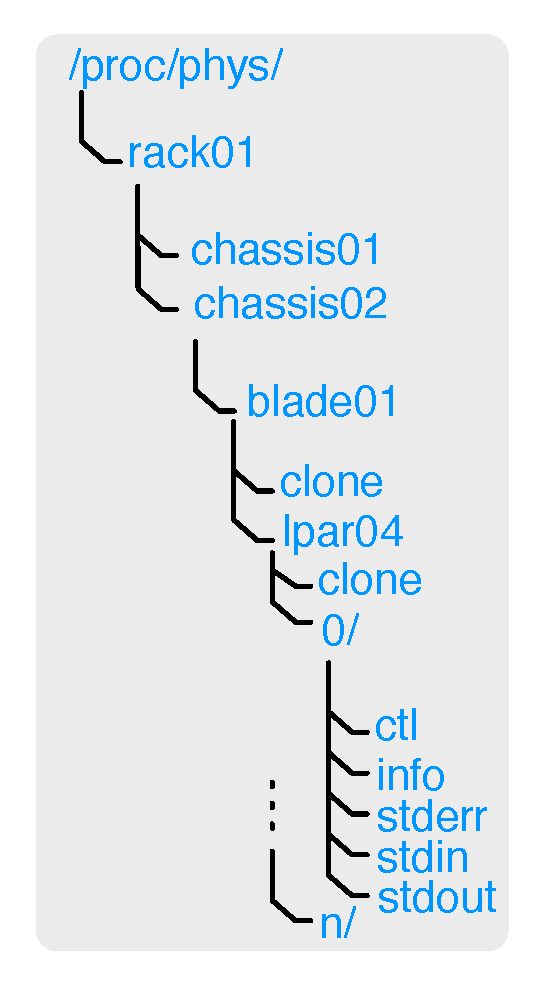
\epsfig{file=ILLUSTRATIONS/org1-phys.eps, width=1.0in}}\hspace{0.1in}
\subfigure[Mimic network topology.]{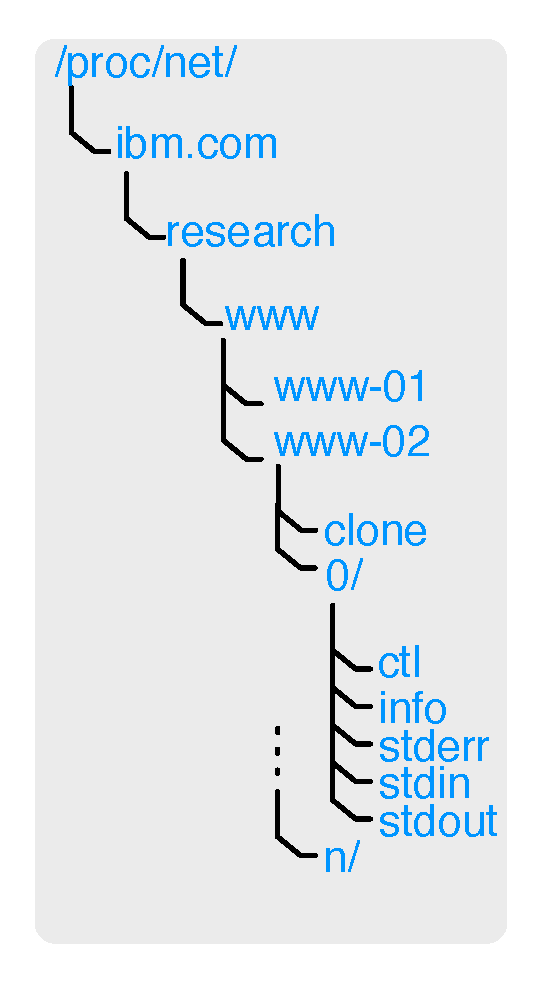
\epsfig{file=ILLUSTRATIONS/org1-network.eps, width=1.0in}}\hspace{0.1in}
\subfigure[Based on resource user.]{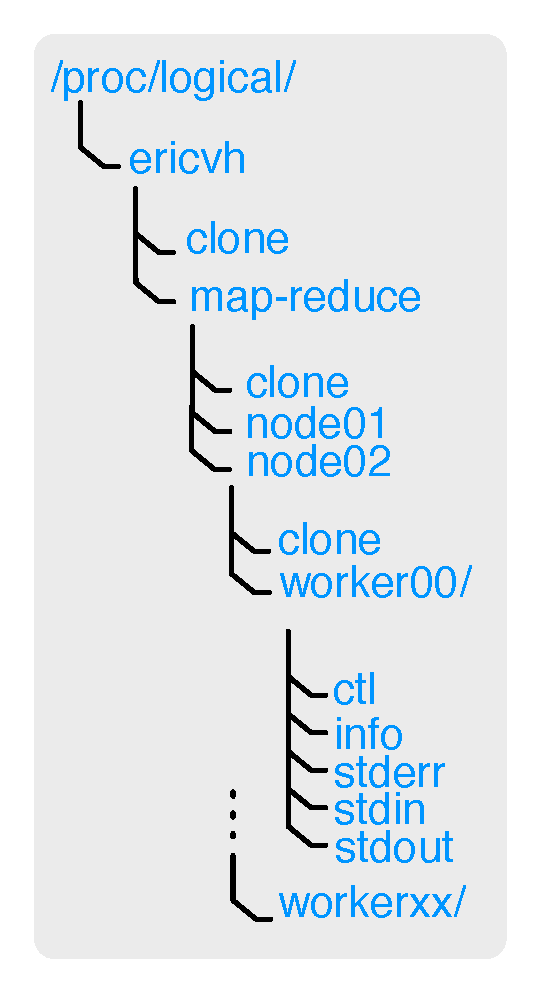
\epsfig{file=ILLUSTRATIONS/org1-logical.eps, width=1.0in}}
\vspace{-0.1in}
\caption{Three examples of organizational views for UEM synthetic filesystem interfaces.}
\label{fig:org-view}
\end{figure}

The cloud computing systems at which UEM is targeted contain on the order
of tens of thousands of computing nodes. 
The size of these systems necessitates
careful consideration of scalability with regards to a synthetic filesystem
interface; a single flat organizational structure will simply not scale.
A viable approach is
the use of a hierarchical structure matching the physical organization of the
nodes (Figure~\ref{fig:org-view}(a)).
A related model would be to use network topology in order to address
resources (Figure~\ref{fig:org-view}(b)).
The nature of either of these hierarchical organizations provides natural
points for aggregation, allowing deployment of UEM ``concentrators'' which
offset scalability issues in monitoring and provisioning 
infrastructures~\cite{evh2008mtags}.
Yet another model would be to use a logical topology based on characteristics
such as the account using the resources, task names, etc.  
(Figure~\ref{fig:org-view}(c)).

In practice, any chosen organizational structure will not be
optimal for every type of access.   
To support dynamic and user-defined organizations, the UEM architecture
is based on
a multi-dimensional semantic filesystem hierarchical structure.
Instead of a single hierarchy, UEM provides access to as many different
hierarchical organizations as make sense for the end user, supporting
physical, logical, network, or other user-defined views.
This multiple-view facility is enabled through a key/value tagging mechanism for
individual leaf nodes. In the synthetic subdirectory corresponding to each process
managed by the UEM are five entries---{\tt ctl}, {\tt info}, {\tt stdin}, {\tt stdout} and {\tt stderr}.
Tags are applied or modified via messages written to a node's {\tt ctl} file
and are reported as part of the {\tt info} file.
These generic tags can then be used by organization and policy
modules to provide structured views into the resources based on relevant
attributes.
This solution works with both physical resources as well as user-defined tasks 
and logical resources.

% Taken out because we don't have space to explain it properly
%The different hierarchies will be accessible from a top-level ``root''
%directory and with proper application of private dynamic namespaces may be
%customized to individual users via system and user-defined scoping rules which 
%may restrict the presented information and views to those of appropriate
%interest to the user which is accessing them (such as through a shortcut name
%like specifying mine instead of using your account name, or using localhost instead
%of specifying the full hostname in a network topology).  
%Furthermore, the application of dynamic scoping semantics to filesystem 
%traversal may be useful at low levels of the hierarchy.
%For example, within a leaf node directory we can provide
%a subdirectory which when traversed will perform resource lookup based
%on the scope of the current level of the hierarchy.  This could be used
%to find a node within the current logical group which has a certain
%resource available, or be used to provide flat access to all processes
%within the current logical group.
%
%TODO: Example is required here.

\begin{figure}
\begin{center}
\begin{verbatim}
 % ls /proc/query/x86/gpus=1/mem=4G
 # will return a list of physical systems matching
 0/
 1/
 2/
 % echo kill > /proc/query/user=ericvh/ctl
 # will terminal all LPARs and/or threads belonging 
 # to user ericvh
 % echo cat /proc/query/os=linux/status
 # returns status of all Linux logical partitions
 node01 up 10:35, 4 users, load average: 1.08 
 node02 up 05:23, 1 users, load average: 0.50
 node03 down
 ...
\end{verbatim}
\end{center}
\vspace{-0.1in}
\caption{Semantic query hierarchy example.}
\label{fig:query}
\end{figure}

\subsection{Dynamic namespace views}
Synthetic filesystems may also enable more dynamic uses of a path to
access resources. For example, the act of accessing a path might be used
to initiate (and determine the search terms of) a search, in a manner similar to a 
RESTful web queries.
A top level query-view may thus be provided by a module, allowing end-users
and applications to embed attribute regular expressions into the filesystem
paths.
This would permit searching for resources with certain capabilities, possibly with partial matches.
It would also permit searches based on 
the current state of resources, as captured, e.g., in the {\tt info} entries
of processes managed via UEM.

If the path in a query corresponds to a directory, a read will
return a directory listing composed of leaf nodes matching the query.  When
a query-path no longer matches any nodes, a file-not-found-error will be returned.
An alternate top-level hierarchy will be provided for users who wish to block
on traversing a query-path until a resource becomes available.  Examples
can be seen in Figure~\ref{fig:query}.

\begin{figure}
\begin{center}
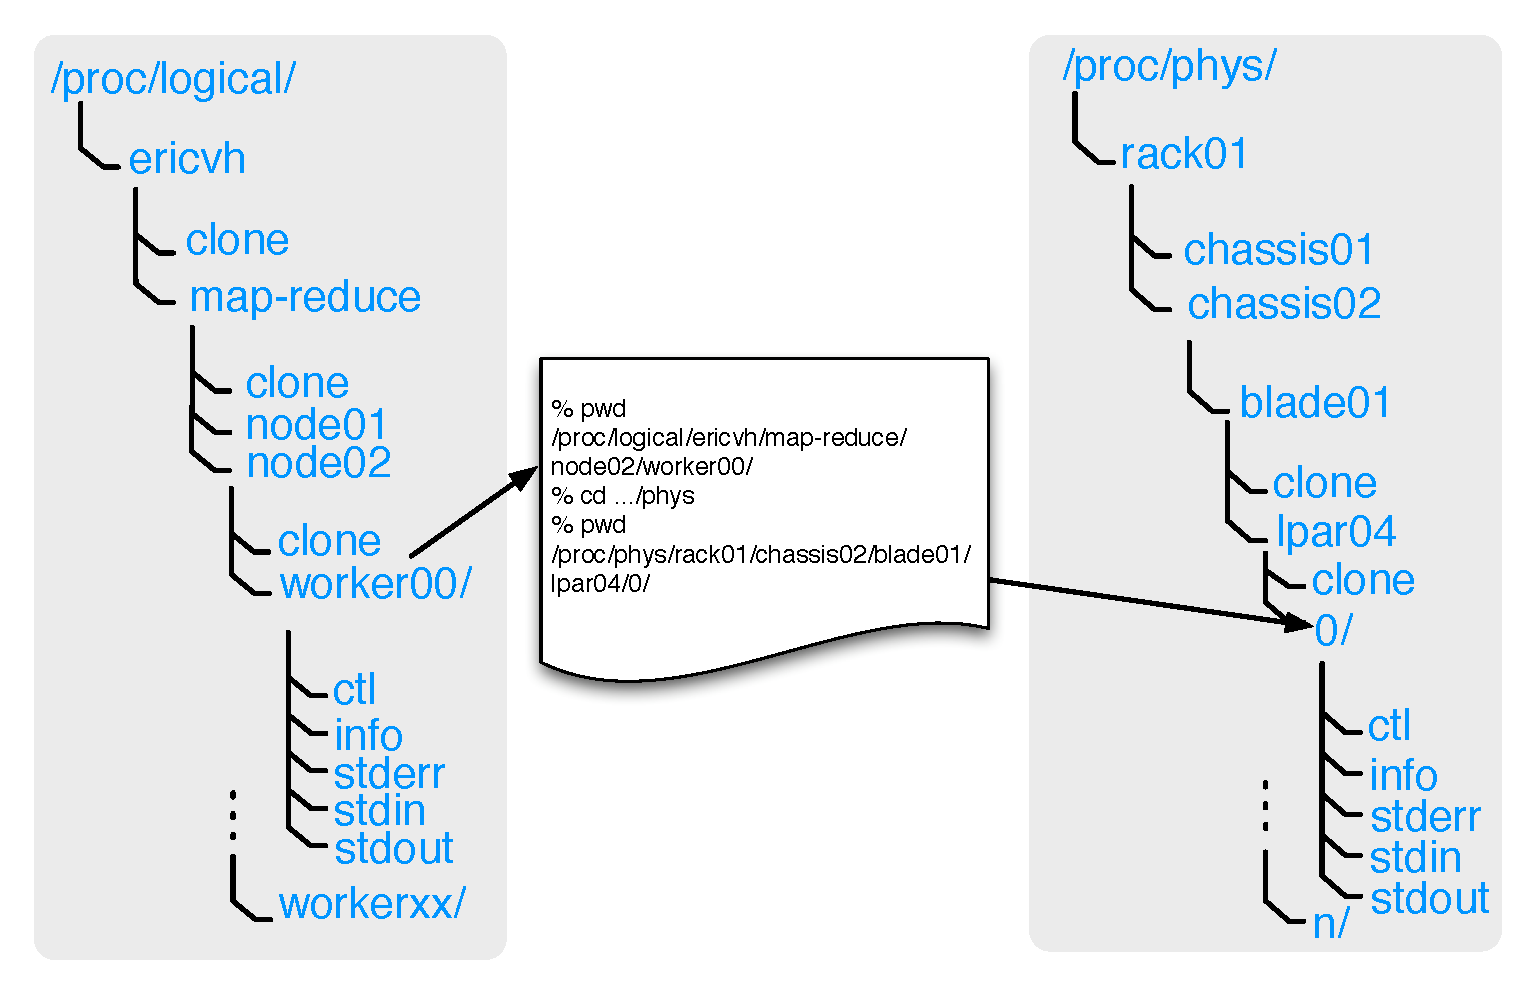
\includegraphics[width=3.4in, keepaspectratio]{ILLUSTRATIONS/org2-dotdotdot.eps}
\end{center}
\vspace{-0.1in}
\caption{Using dot-dot-dot to shortcut from one hierarchy to another.}
\label{fig:dot-dot-dot}
\end{figure}


In addition to switching between views of a hierarchy (as seen from the hierarchy's root), it
is also useful to be able to change views while at a navigation point
{\it within} the hierarchy, without losing the implicit state associated
with the current position in a synthetic filesystem hierarchy.

One possible approach is to define a semantic filesystem shortcut, henceforth
referred to as {\it dot-dot-dot} (Figure~\ref{fig:dot-dot-dot}), 
which allows users to switch semantic views while maintaining context of 
their existing location.  In Figure~\ref{fig:dot-dot-dot}, the dot-dot-dot shortcut is used to switch between
the logical view and the physical view while maintaining the context of the 
current process.  This mechanism could also be used to allocate a new thread (or even a
logical partition) on the same physical machine of an existing thread.

Given the presence of many different views of the organizational hierarchy of
a system,
it will be necessary to have a single canonical view of the hierarchy in which
all nodes see the same leaf nodes at the same location.
This is necessary both for use by administrative tools which might require
a more static view of the resources as well as to be able to communicate
path-based references to particular resources.  This will be particularly
important in order to establish an abstract addressing model for I/O and
communication.  Devising a meaningful canonical view that meets these
criteria is one of our ongoing efforts.

\subsection{Policy}
\label{section:policy}

The allocation of resources is controlled by policy modules.  Physical
allocation policy modules are by far the most simple, providing reservation 
based access to physical resources.  The logical policy modules are built 
on top of the physical policy modules, allocating virtual machines 
and/or tasks on top of pre-allocated physical or logical resources.
The default policy modules provide a space-based partitioning model which 
allows for simple logical node allocation and task deployment with each
task getting its own logical node.  

While we provide default allocation policy modules, the UEM
is not limited to a single policy.  Users and/or administrators may
define their own policy modules which can make provisioning decisions 
based on machine constraints, resource load, quality of service
contracts, or external quantitative influences such as who is willing
to pay more for the service.   These user-defined policy modules can
govern any subset of resources and may be deployed at different levels
of the organizational hierarchy.

Beyond allocation based policies, users or administrators may deploy
monitoring agents and runtime policy modules throughout the infrastructure
using the same execution methodology they would use to deploy tasks.
Policy agents may also operate directly on the UEM synthetic file hierarchy,
gathering and aggregating monitoring information and (infrastructure
permitting) reorganize resources and task execution location to optimize for
power efficiency, bandwidth, cost or other factors.

\subsection{Execution}
The mechanism behind initiating execution is based on 
XCPU's example of using a synthetic file (conventionally named {\tt clone},) with special semantics, 
to allocate new resources.
Clone files are used in the Plan 9 operating system's synthetic file servers
to atomically allocate and 
access an underlying resource.

%%  PSM: the following isn't really relevant here:
%%  
%%  Their most common use is found in the
%%  Plan 9 networking stack, where they are used both to allocate protocols
%%  on network devices, and communication channels (such as sockets) within
%%  protocols.  

An {\tt open()} system call on a {\tt clone}
file doesn't return a file descriptor to the (synthetic) {\tt clone} file itself.  
Instead, a new synthetic subdirectory is created to represent the resource
containing control/status files for that instantiated resource.
The file descriptor returned from opening the {\tt clone} file points to a 
control file (conventionally named {\tt ctl},) within the newly allocated subdirectory so that the 
application/user can directly interact with the resource they just 
allocated.  All the resources allocated by the initial opening of the
{\tt clone} file are
released and garbage-collected when the user/application closes the {\tt ctl} 
file. 

For example, a new task can be initiated by opening the {\tt clone}
file in the UEM {\tt /proc} filesystem, using a path, as described
in Section~\ref{section:organization}, to describe the required resources.
Such an operation will initiate interaction with relevant policy modules to reserve the required resources,
if available, and return a handle to a {\tt ctl} file. 
In a fashion similar to Plan 9's \emph{cpu} command, it will also 
export local resources such as the filesystem, standard input, output, and 
the user's current shell environment, to the newly allocated resources.
Following the convention of Inferno's devcmd~\cite{inferno:man} and XCPU, we 
initiate execution by writing a command to the open {\tt ctl} file handle 
detailing the (local) path to the executable and command line arguments.
Other configurations, such as alternate namespace configuration, environment
variables, etc., can be specified either through direct interaction with the
control file or through other filesystem interfaces.
The remote node will then setup the namespace and environment and initiate
execution of the application, redirecting standard I/O to the originating 
user context (unless otherwise specified as mentioned later in Section~\ref{section:communication}).  Since this same interface is available on every node of the system,
subsequent task executions can be triggered from within the cluster providing 
a much more dynamic environment than is available in many of today's cluster
workload management systems.

\subsection{Configuration}
The same approach as taken for initiating execution can be used to provision a logical node or 
other resource within a cluster.  Instead of an application binary, a disk
image or an XML virtual machine specification may be passed in the commands being sent to
a {\tt ctl} interface in the UEM namespace.  In the case of logical nodes, standard I/O handles in the file
system are hooked to the console of the virtualized system.
Simply allocating a logical node on a particular piece of physical hardware
is somewhat less compelling.
Instead we take advantage of the dynamic aspects of the 
query hierarchy to help allocate machines with specific
attributes (i.e., {\tt /cloud/x86/gpus=1/mem=4G/clone}) without having to specify
a physical node.  The same technique could be a general mechanism to find 
hardware capable of supporting the objtype for a given application 
(or allocating new logical nodes on demand as necessary if none are currently
available).

A variation of this attribute specification can be used to allocate
a cluster of nodes (i.e., {\tt /cloud/x86/gpus=1/mem=4G/num=16/clone}).
In the case that insufficient physical resources are available to 
satisfy a logical (or physical) node request a file not found error 
message will be provided back to the provisioning user or application.
As mentioned earlier, doing directory listings at any level of the attribute 
query semantic hierarchy will detail available nodes matching the 
classification and the user can use the blocking query hierarchy to wait
for resources to become available. 

In the case of a group allocation, opening the {\tt clone} file allocates 
a new node subdirectory which actually represents the set of nodes 
allocated.  In addition to
control and status files which provide aggregated access to the individual
logical nodes, it will provide subdirectories for each of the logical 
nodes allocated providing individual access and control.  Commands sent to 
the top level control file will be broadcast to the individual nodes 
(allowing, for instance, them to all boot the same disk image).  
We are refining the syntax of the control 
commands on these meta files to allow for certain
keywords which enable necessary differentiation (specifying for instance
individual copy-on-write disk images and network MAC addresses).
This same approach can be used to launch a set of processes on many remote
nodes to perform a scale-out operation such as MapReduce workloads or
Monte Carlo simulations.

%Such a model might have multiple clone files at
%multiple levels providing abilities to instantiate new logical nodes, logical
%partitions, or threads.
% TODO: This needs to be reworked to fit here and expanded into a better
% example
% TODO: May be better presented in a semantic filesystem subsection
% this is an extension of clone to create logical organizational spaces
% as well as new logical partitions and threads.
%Perhaps the most flexible approach would be to allow users to define an
%arbitrary hierarchical organizational structure using a /n-like dynamically
%generated organization terminated by a clone file to allocate resources at
%that level of the hierarchy.  

% Plan 9 specific arguments in the next two paragraphs
%The use of clone files to instantiate threads may be a bit controversial
%as it always comes up as the example of how we don't want to use a file
%system for everything.	However, I believe the need for distributed
%execution contexts trumps prior reasons for not instantiating new threads
%through a filesystem interface.  Its not clear that there should be a
%complete switchover to using filesystem operations for things such as
%fork, but it seems clear that we need an architected mechanism for
%execution in other contexts.  By using a synthetic filesystem for
%this interface, it means we can easily export it to other environments --
%all the system would need is a 9P client library or filesystem in order
%to access the execution model.
%
%For example -- Inferno and Plan 9 have different files based on what
%underlying information and controls are available.  Given the wide
%space we intend to address, this will likely be the case for us as well.

\subsection{Communication}
\label{section:communication}
% TODO: maybe reformat this to be more of a lead-in to PUSH
%Communication and coordination of different instances of the execution
%model will be accomplished via a single pipe.  Client and Server messages
%will be sent on the same pipe, with a special mux on either end capable of
%distributing requests or responses as appropriate.  This will allow
%communication between two hosts when only one of the hosts is addressable,
%it will also allow easier tunneling of communication paths.  Extensions on
%this mux to allow bridging of network domains will also have to be investigated.

%The idea is that this could provide a more dynamic execution
%model for EC2 deployments of Plan 9 and Inferno as well as
%provide the foundation for large scale deployments of applications
%as part of the DOE HARE project.  This should also fill the distributed
%execution requirements for the PUSH project (which in turn will provide
%facilities for connecting distributed execution in a pipeline fashion).

The UEM takes the UNIX idea of linking processes together with
local pipelines and generalizes it to distributed systems by allowing
file descriptors to be managed from within the synthetic filesystem 
control interfaces.
This allows the composition of distributed workflows out of simple
sets of tools designed to do one thing well.
Establishing a UNIX-style pipe between a local and remote task is
straightforward, since the local standard I/O context (the {\tt stdout} synthetic file) is exported
to the remote task which accesses it directly.  Attempting to establish a deep multi-stage
pipeline is however more complex, as it is undesirable for all I/O between stages to flow through the
initiating node.
To avoid this, file descriptors in UEM can be redirected {\it directly} between nodes executing 
the stages of the pipeline, with the redirection initiated through the UEM control interface ({\tt ctl} files).  This is particularly important for long pipelines
and for fan-out workflows.

%This allows users to specify communication pipelines between distributed
%tasks without routing the
%By doing this, users can 
%not only instantiate new tasks on 
%remote nodes, they can specify communication channels between these
%tasks without the need to employ an external message passing infrastructure.
%By specifyin
%As with the UNIX process model and its standard sets of inputs
%and outputs it is possible to compose workflows
%out of simple sets of tools designed to do one thing well.

\begin{figure}
\begin{center}
\begin{verbatim}
 # proc102 | proc56 | proc256
 # usage: splice <proc_path> <src_fd> <local_fd>
 % echo splice /proc/net/remote.com/102 1 0 \
    > /proc/net/mybox.com/56/ctl
 % echo splice /proc/net/mybox.com/56 1 0 \
    > /proc/net/farther.com/256/ctl
\end{verbatim}
\end{center}
\vspace{-0.1in}
\caption{Creating a three-way distributed pipe using UEM.}
\label{fig:splicex}
\end{figure}

This approach is best illustrated by an example. Assume that we
want to run a three-stage pipeline with each process (process IDs
102, 56 and 256) residing on a separate system ({\tt remote.com}, {\tt mybox.com}
and {\tt farther.com}). We assume that the processes have already been
instantiated via the UEM interface.  The operation of splicing
the I/O can be seen in Figure~\ref{fig:splicex}.  The splice command
takes three arguments: the canonical path to the source process, the 
file descriptor number within the source process, and the target file
descriptor within the local process we wish to stream the source into. 

\begin{figure}
\begin{center}
\begin{verbatim}
push -c '{
  ORS=./blm.dis
  du -an files |< xargs os \\
   chasen | awk '{print \$1}' | sort | uniq -c \\
   >| sort -rn
\end{verbatim}
\end{center}
\vspace{-0.1in}
\caption{Examples of {\it fan-out} and {\it fan-in} with the PUSH shell.}
\label{fig:push}
\end{figure}

% OLD START
Tying all this together is a new shell, named PUSH~\cite{PODC:Push}, which 
uses the facilities of the UEM to allow pipelining of 
distributed computation.  The central goal of PUSH is to provide shell 
abstractions for the capabilities of UEM that provide a language-independent, 
terse, and simple way of instantiating large distributed jobs 
that are traditionally performed by middleware in modern {\it data intensive 
supercomputing (DISC)} systems. 
PUSH provides {\it fan-out}, {\it fan-in}, and {\it hash-pipe} operators 
providing map, reduce, and all-to-all communication mechanisms between
pipeline stages.
User-defined modules can be specified to 
decompose and reconstitute byte streams into records and back into byte 
streams again, allowing output from one process to go to many and vice 
versa.
% END OLD START

%The process takes place as follows:
%First we splice remote.com to localhost. we do this by informing
%the localhost standard input control file, \\
%/proc/localhost/56/fd/0/ctl,
%of its new target. This is done by giving the control file a ``splice''
%command telling it the data source in this case
%/proc/net/remote.com/102/fd/1/data. We do the same thing to farther.com,
%splicing \\
%/proc/net/mybox.com/56/fd/1/data to \\
%/proc/net/farther.com/256/fd/0/ctl.

%a scope-driven hierarchy (a level for logical nodes, a level beneath
%that for processes on those nodes (perhaps several different classes
%of levels beneath logical nodes representing different types of thread
%(limbo, native host, or emulated).  The idea would be the same
%interface for local, remote, or hosted (in the case of Inferno) (or
%emulated in the case of CNK on BG/P).	Push could then interact
%directly with this hierarchy to deploy threads.  Another side-aspect is
%alternate views -- the hierarchical layout is the canonical form, but
%there may be other views which can be obtained which make more logical
%sense (ie. nodes/threads associated with a user, a task, or whatnot),
%the other ``requirement'' would be for some sort of cluster-based
%allocation as opposed to just individual node (ie. start up 100 nodes,
%each running 4 threads of this executable).  While this could be
%incorporated into the ctl interface (as it is on XCPU to some extent),
%it might be nice to be able to do such an operation in a cluster view,
%but then be able to access the individual threads in the user-view or
%the canonical view.


\section{Case Study}
\begin{figure}
\subfigure[]{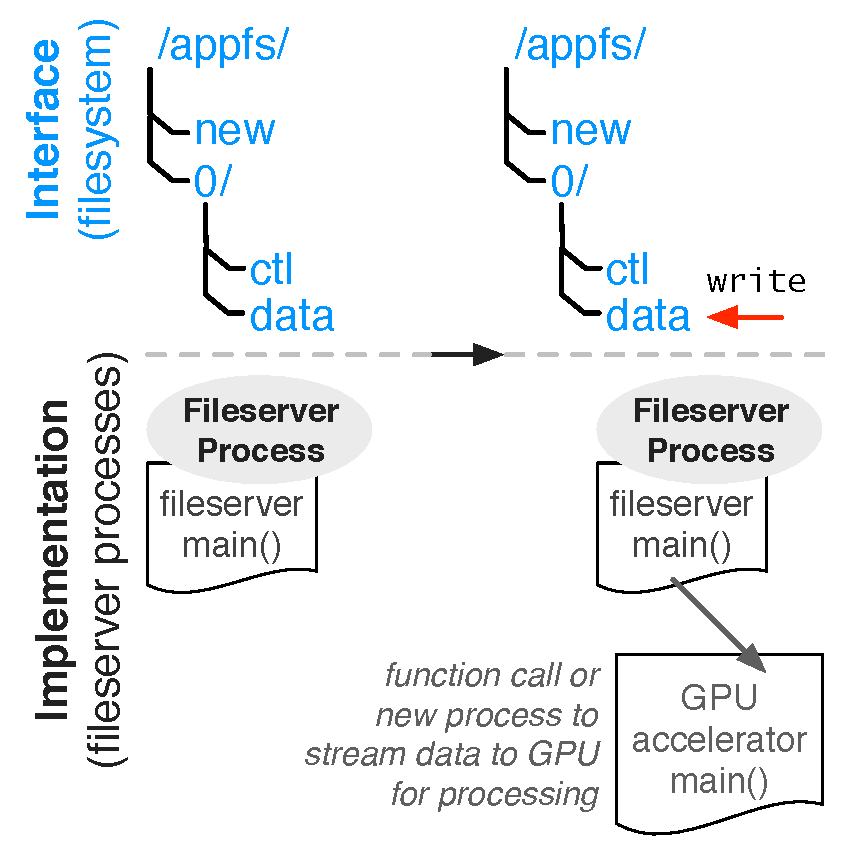
\epsfig{file=ILLUSTRATIONS/time-evolving-filesystems-a.eps, width=1.5in}}\hspace{0.1in}
\subfigure[]{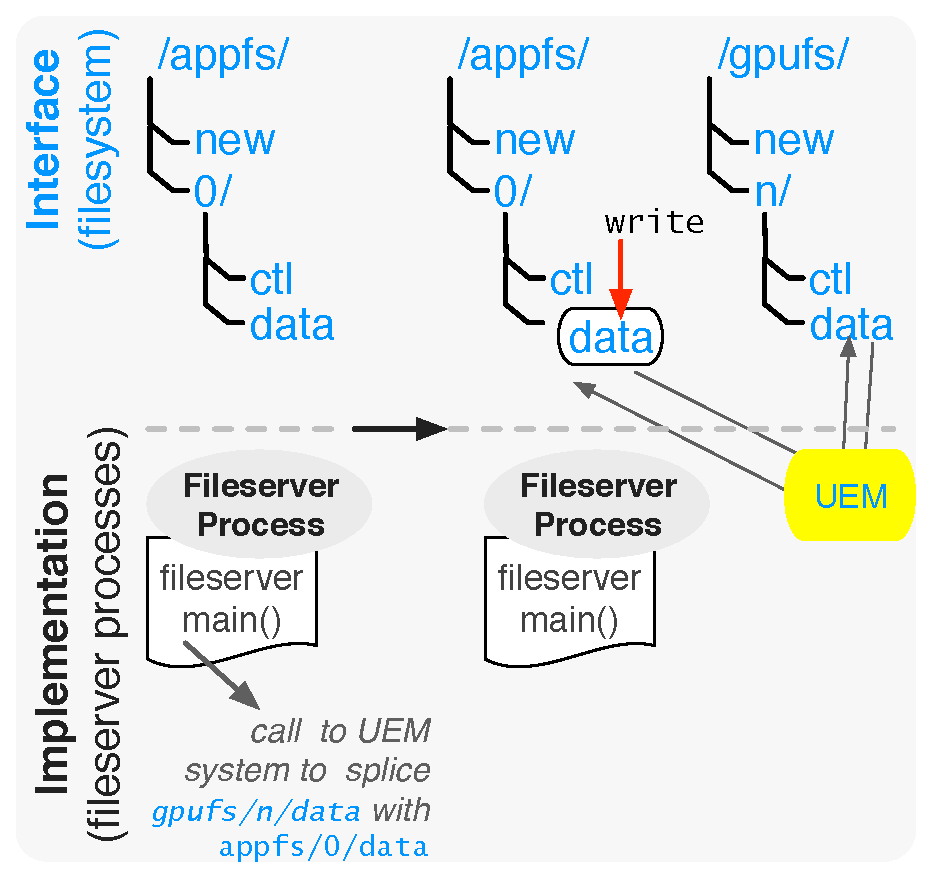
\epsfig{file=ILLUSTRATIONS/time-evolving-filesystems-b.eps, width=1.7in}}
\vspace{-0.1in}
\caption{Illustration of time-evolving dynamic synthesized filesystems.}
\label{fig:dynamicnamespace}
\end{figure}
One example application of the UEM is in systems that themselves
use synthetic filesystems for representing interfaces to compute
or communication resources. If, in such systems, new entries in the
served namespace may be dynamically created, or if new interactions
between existing entries may occur (Figure~\ref{fig:dynamicnamespace}),
static approaches to interfacing and interconnection will be insufficient.

The Sunflower full-system simulator for networked embedded
systems~\cite{StanleyMarbell:hipeac07} provides one illustration
of such a system. Sunflower is a microarchitectural simulator
intended for use in modeling large networks of embedded systems.
Due to the tension between the computation requirements of the
instruction-level hardware emulation it performs, and the desire
to emulate hardware systems comprising thousands of complete embedded
systems, it implements facilities for distributing simulation across
multiple {\it simulation hosts}. To facilitate distributed simulation,
Sunflower includes built-in support for launching simulation engines
on Amazon's EC2. Each of these individual simulation engine instances
executes as a filesystem server~\cite{StanleyMarbell:iwp906a},
serving a small hierarchy of synthetic interface files for interacting
with the simulation engine instance and the resources simulated
within the engine instance.

\subsection{Distributed simulation in Sunflower}
Each simulation host taking part in a distributed simulation in
Sunflower exposes its modeled resources and control interfaces
as a dynamically synthesized filesystem (Figure~\ref{fig:in-network-splicing}(a)).
Through this interface, it is possible to access all the state
(processor state, network packets, modeled analog signals, etc.) within
components of the system modeled at a given host.  When executing
a distributed simulation, a central {\it interface host} connects
to each host filesystem, and launches multiple concurrent threads
to cross-connect the exposed interfaces to achieve a single system
(Figure~\ref{fig:in-network-splicing}(b)). For example, by
cross-connecting (by continually reading from one and writing to the other)
the {\tt netin} and {\tt netout} of multiple
simulation engines (on possibly-different simulation hosts, e.g.,
hosts 1--4 in Figure~\ref{fig:in-network-splicing}(b)), the simulated
interconnects in the systems are unified.  The central host
also ensures the coherent evolution of time across these different
simulation hosts, by implementing algorithms from the
domain of parallel discrete-event simulation.

\begin{figure}
\subfigure[]{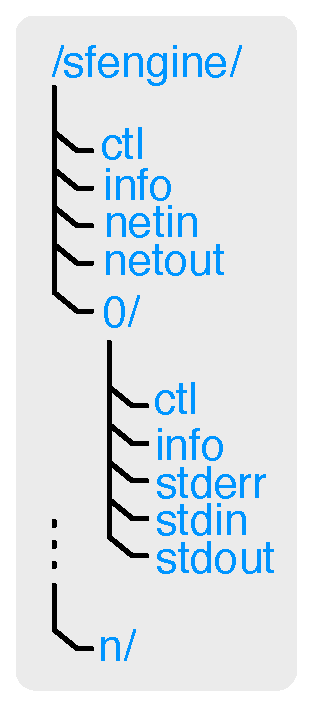
\epsfig{file=ILLUSTRATIONS/sunflowerfs.eps, height=1.6in}}\hspace{0.25in}
\subfigure[]{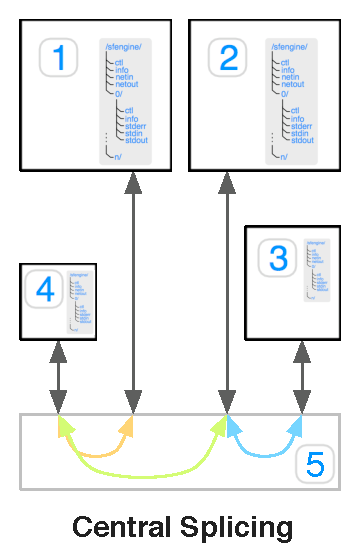
\epsfig{file=ILLUSTRATIONS/in-network-splicing-a.eps, width=1.0in}}\hspace{0.25in}
\subfigure[]{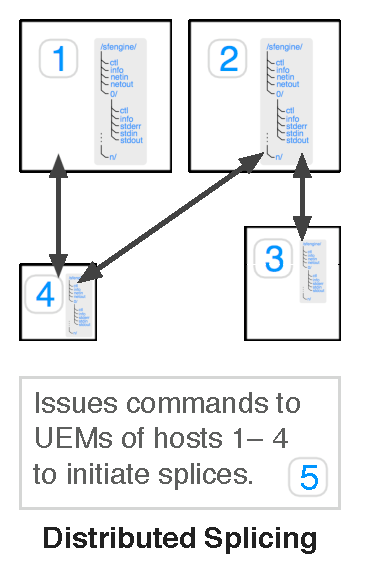
\epsfig{file=ILLUSTRATIONS/in-network-splicing-c.eps, width=1.0in}}
\vspace{-0.1in}
\caption{Illustration of potential for removal of the central
inter-interface splicing facilitated by the unified execution
model's in-network streaming. The filesystem interface at each
of the five hosts (four simulation hosts and one control interface),
is shown in (a).}
\label{fig:in-network-splicing}
\end{figure}

\subsection{Distributed splicing with UEM}
In-network splicing in UEM, as described in
Section~\ref{section:communication}, provides a way for cross-connection
of file descriptors within a hierarchy of files, with the
cross-connection (splicing) occurring on one of the nodes involved
in the splice, and with the {\it splicing facilitated transparently
by the system}. Thus, for example, rather than having to execute
processes to stream data between the file interfaces to the modeled
interconnect between the node pairs (1, 4), (2, 4) and (2, 3) (by
cross-connecting the {\tt netin} and {\tt netout} interfaces with
processes that continually stream data), the central control interface
only needs to {\it initiate} the cross connection between these
pairs (Figure~\ref{fig:in-network-splicing}(c)). This can be done using the mechanism
described in Section~\ref{section:communication}, Figure~\ref{fig:splicex}.


\subsection{Dynamic call chains with UEM}
The interaction between multiple hosts' simulation engines may go
beyond static interconnections such as those described thus far.  Per-host statistics tracers
may, for example, be triggered to commence detailed logging of
network traces or architectural state based on time or machine-state
information. This could lead to {\it fileservers within a UEM filesystem
triggering the instantiation of new fileservers}. Thus, although a
simulation of a particular system will typically involve the creation
of an initial static distributed filesystem of simulation state,
further work may be triggered by this filesystem at runtime.  

\section{Discussion}
This article presented the architecture for a {\it unified execution model (UEM)} for structuring the provisioning, and runtime usage of large dynamically
changing collections of computing systems, as is typical of so-called
cloud computing systems.

By leveraging user- and system-provided policy, monitoring  and organizational 
modules that interface to the UEM, the UEM is extensible, allowing exploration of alternate 
organizational models, scheduling and resource allocation policies. This will hopefully 
facilitate new ways of interacting with the dynamic distributed resources 
which today's cloud computing infrastructures provide.

In addition to the topics covered in this article, we are also actively
investigating the application of the UEM to hybrid computing environments
with GPU and Cell Processor based accelerators~\cite{evh2009ppac}. 
We are also investigating its application on extreme scale high performance 
computing systems such as BlueGene and Roadrunner~\cite{evh08hare}.
At extreme scale, we are exploring methods of aggregating monitoring, 
command, and control of the resources providing logical grouping models for
system services and automated workload rebalancing and optimization.
%~\cite{evh2008mtags}.  
Another area of active investigation is determining
mechanisms for providing fault-tolerance both within our infrastructure and
for application tasks which are deployed by it.

The true potential of cloud computing systems will only
be realized when cloud interfaces and management mechanisms 
are integrated into end-user environments as well as the applications
themselves.
The importance of the consolidated interface that the UEM embodies is that it 
permits the organization and orchestration of computing resources in a logical
manner, maintaining a holistic view of the distributed system.
The use of synthetic semantic filesystems enables the creation of a
co-operating environment which isn't tightly bound to a particular 
operating system, programming language, or runtime system; this facilitates its use on legacy
and heterogeneous systems, such as those containing computing accelerators
(e.g., GPUs or dedicated hardware such as cryptographic encoder/decoders).
Providing interfaces for allocating new resources as well as integrated mechanisms 
to deploy and connect tasks on those resources is the first step towards cloud 
enabling applications and workflows providing new degrees of flexibility, efficiency,
reliability, and productivity.

\section{Acknowledgements}

This work has been supported in part by the Department of Energy Office of
Science Operating and Runtime Systems for Extreme Scale Scientific
Computation project under contract \#DE-FG02-08ER25851.

%
% The following two commands are all you need in the
% initial runs of your .tex file to
% produce the bibliography for the citations in your paper.
\bibliographystyle{abbrv}
\bibliography{brasil} % sigproc.bib is the name of the Bibliography in this case
\end{document}
